\documentclass[a4paper, fontsize=12pt]{article}
\input ../../my_simple_preamble.tex
\usepackage{pgfplots}
\pgfplotsset{compat=1.15}
\usepackage{mathrsfs}
\usetikzlibrary{arrows}

\begin{titlepage}
    \title{Контрольная №1}
    \author{Морозов Н.Ю. 23.Б09}
    \date{}
\end{titlepage}

\begin{document}

    \definecolor{cqcqcq}{rgb}{0.7529411764705882,0.7529411764705882,0.7529411764705882}
    \maketitle  
        
    \section{}

    $ \sphericalangle \quad f : A \longrightarrow B,\ |A| = k,\ |B| = n$ при $ k \leqslant  n $ только в этом случае возможна иньекция. 

    \noindent Пусть N - искомое количество возможных отображений из $A$ в $B$, тогда

    \begin{enumerate}
        \item N $= A^k_n$, что справедливо для любых $n, k \in \mathbb{N}, \{0\} $ удовлетворяющих условию.
        \item Также это будет верно и для тех случаев когда оба множества пустые и когда $A - \varnothing $, а $B$ - любое
        конечное, поскольку эти случаи соотвестуют условиям выше.
        \item А для случая $A$ -- любое конечное, но не пустое, $B - \varnothing$  не выполняется неравенство 
        $ k \leqslant  n \Longrightarrow f -$ не иньекция $\Longrightarrow$ этот случай не подходит.
    \end{enumerate}

    \section{}

    Mорозов $ \Longrightarrow $ N = 7

   \noindent $E_i$ -- матождиание для события вытащено $i$ тузов.

   

    \begin{align*}
        &E = \sum_{i = 0}^{4} \left(\frac{C^{7-i}_{32} \cdot C^{i}_{4}}{C^7_{36}} \cdot i \right)  =
        \sum_{i=0}^{4} \left( \frac{\frac{32!}{(7-i)!(32-7+i)!} \cdot \frac{4!}{i!(4-i)!}}{\frac{36!}{7!(36 - 7)!}} \cdot i\right)  = \frac{7}{9}\\
        &D = \sum_{i=0}^{4} \left( \frac{\frac{32!}{(7-i)!(32-7+i)!} \cdot \frac{4!}{i!(4-i)!}}{\frac{36!}{7!(36 - 7)!}} \cdot i^2\right) - \left(\frac{7}{9}\right)^2 = \frac{232}{405}
    \end{align*}

    \section{}

    \begin{enumerate}
        \item $34816572 = 34816725$
        \item $34816725 = 34816752$
        \item $34816752 = 34817256$
        \item $34817256 = 34817265$
        \item $34817265 = 34817526$
        \item $34817526 = 34817562$
        \item $34817562 = 34817625$
        \item $34817625 = 34817652$
    \end{enumerate}

    \newpage

    \section{}

    \begin{figure}[ht]
    \centering
    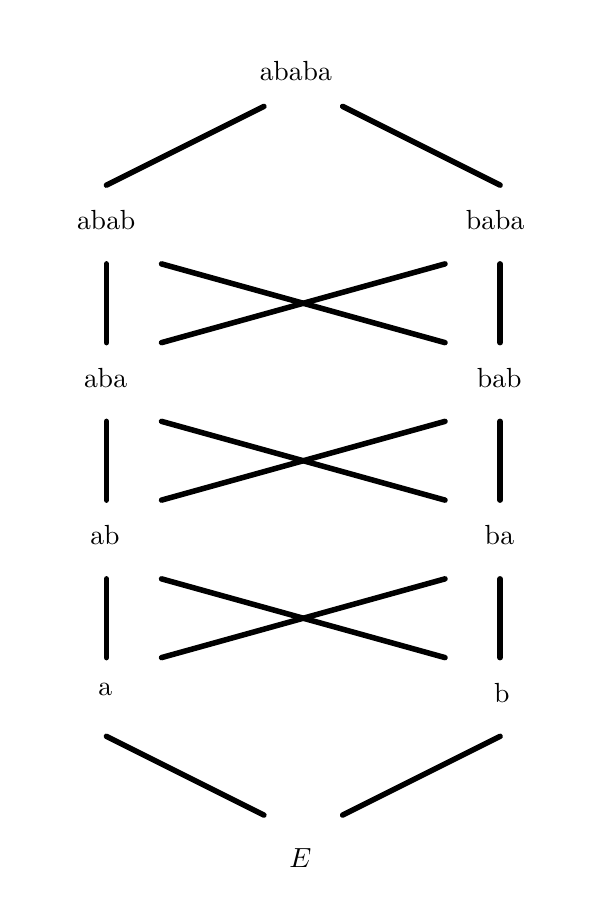
\begin{tikzpicture}[line cap=round,line join=round,>=triangle 45,x=1.0cm,y=1.0cm]
        \clip(7,-7) rectangle (14.00,4);
        \draw (9.82,3.7) node[anchor=north west] {ababa};
        \draw [line width=2.pt] (10.,3.)-- (8.,2.);
        \draw (7.5,1.8) node[anchor=north west] {abab};
        \draw [line width=2.pt] (8.,1.)-- (8.,0.);
        \draw (7.59,-0.2) node[anchor=north west] {aba};
        \draw [line width=2.pt] (8.,-1.)-- (8.,-2.);
        \draw (7.67,-2.2) node[anchor=north west] {ab};
        \draw [line width=2.pt] (8.,-3.)-- (8.,-4.);
        \draw (7.77,-4.2) node[anchor=north west] {a};
        \draw [line width=2.pt] (8.,-5.)-- (10.,-6.);
        \draw [line width=2.pt] (11.,3.)-- (13,2.);
        \draw [line width=2.pt] (13.,1.)-- (13.,0.);
        \draw [line width=2.pt] (13.,-1.)-- (13.,-2.);
        \draw [line width=2.pt] (13.,-3.)-- (13.0,-4.);
        \draw [line width=2.pt] (13.,-5.)-- (11.0,-6.);
        \draw (10.2,-6.3) node[anchor=north west] {$E$};
        \draw (12.44,1.8) node[anchor=north west] {baba};
        \draw (12.58,-0.2) node[anchor=north west] {bab};
        \draw (12.68,-2.2) node[anchor=north west] {ba};
        \draw (12.8,-4.2) node[anchor=north west] {b};
        \draw [line width=2.pt](8.7,1) -- (12.3,0);
        \draw [line width=2.pt](8.7,0) -- (12.3,1);
        \draw [line width=2.pt](8.7,-1) -- (12.3,-2);
        \draw [line width=2.pt](8.7,-2) -- (12.3,-1);
        \draw [line width=2.pt](8.7,-3) -- (12.3,-4);
        \draw [line width=2.pt](8.7,-4) -- (12.3,-3);
        \end{tikzpicture}
    \end{figure}

\section{}

    \begin{figure}[h]
        \centering
        \begin{tikzpicture}[line cap=round,line join=round,>=triangle 45,x=1.0cm,y=1.0cm]
            \clip(-9.,0.) rectangle (9.,7.);
            \draw (-0.849,6.7) node[anchor=north west] {5б + 5ч};
            \draw (-8.8,6.7) node[anchor=north west] {10ш};
            \draw (-8.8,4.78) node[anchor=north west] {9ш};
            \draw (-8.8,2.78) node[anchor=north west] {8ш};
            \draw (-8.8,0.57) node[anchor=north west] {12ш};
            \draw [line width=2.pt] (-1.,6.)-- (-5.,5.);
            \draw [line width=2.pt] (1.,6.)-- (5.,5.);
            \draw [line width=2.pt] (5.,4.)-- (5.,3.);
            \draw [line width=2.pt,dash pattern=on  4.5pt off 3pt] (5.,2.)-- (5.,1.);
            \draw [line width=2.0pt,dash pattern=on 4.5pt off 3pt] (0.,2.)-- (0.,1.);
            \draw [line width=2.pt] (-5.,4.)-- (-5.,3.);
            \draw [line width=2.pt,dash pattern=on 4.5pt off 3pt] (-5.,2.)-- (-5.,1.);
            \draw (4.153936824635312,4.78) node[anchor=north west] {5б + 4ч};
            \draw (-5.832531296790888,4.78) node[anchor=north west] {4б + 5ч};
            \draw (-5.852464366893535,2.78) node[anchor=north west] {3б + 4ч};
            \draw (4.153936824635312,2.78) node[anchor=north west] {4б + 3ч};
            \draw (-5.852464366893535,0.57) node[anchor=north west] {7б + 5ч};
            \draw (4.153936824635312,0.57) node[anchor=north west] {5б + 7ч};
            \draw (-0.849,0.57) node[anchor=north west] {6б + 6ч};
            \draw (-0.849,2.78) node[anchor=north west] {4б + 4ч};
            \draw [line width=2.pt] (-4.,4.)-- (-1.,3.);
            \draw [line width=2.pt] (4.,4.)-- (1.,3.);
            \draw (-3.26116525354941,6.58) node[anchor=north west] {$\frac{1}{2}$};
            \draw (2.778554987552662,6.58) node[anchor=north west] {$\frac{1}{2}$};
            \draw (2.24036209478119,4.63) node[anchor=north west] {$\frac{5}{9}$};
            \draw (-2.7030392906752922,4.63) node[anchor=north west] {$\frac{5}{9}$};
            \draw (5.40972024110208,3.9) node[anchor=north west] {$\frac{4}{9}$};
            \draw (-5.932196647304123,3.9) node[anchor=north west] {$\frac{4}{9}$};
            \draw (-5.89233050709883,1.9) node[anchor=north west] {$\frac{5}{12}$};
            \draw (0.4065196453376562,1.9) node[anchor=north west] {$\frac{1}{2}$};
            \draw (5.170523399870315,1.9) node[anchor=north west] {$\frac{5}{12}$};
        \end{tikzpicture}
    \end{figure}

    \section{}
\end{document}